\section{Experimental Results}\label{sect:evaluation}

%cost table
\begin{figure}[t]
	\centering
	%\subfloat[Total \shortname gas cost]{
	%		\begin{tabular}[b]{| c | c | c | c | }	
	%			\hline
	%			$n$ &	$\owner$ & Active $\shareholder$ & Passive $\shareholder$
	%			\\	\hline \hline
	%2	&	3.1E-2		$\Xi \left[	5.48	\$ \right] $	&	9.1E-3		$\Xi \left[	1.62	\$ \right] $	&	5.0E-3		$\Xi \left[	0.89	\$ \right] $
	%\\ \hline
	%3	&	3.3E-2		$\Xi \left[	5.80	\$ \right] $	&	9.2E-3		$\Xi \left[	1.63	\$ \right] $	&	4.8E-3		$\Xi \left[	0.85	\$ \right] $
	%\\ \hline
	%4	&	3.4E-2		$\Xi \left[	6.11	\$ \right] $	&	9.2E-3		$\Xi \left[	1.64	\$ \right] $	&	5.1E-3		$\Xi \left[	0.91	\$ \right] $
	%\\ \hline
	%5	&	3.6E-2		$\Xi \left[	6.43	\$ \right] $	&	9.3E-3		$\Xi \left[	1.65	\$ \right] $	&	5.2E-3		$\Xi \left[	0.92	\$ \right] $
	%\\ \hline
	%6	&	3.8E-2		$\Xi \left[	6.75	\$ \right] $	&	9.4E-3		$\Xi \left[	1.66	\$ \right] $	&	5.2E-3		$\Xi \left[	0.93	\$ \right] $
	%\\ \hline
	%7	&	4.0E-2		$\Xi \left[	7.07	\$ \right] $	&	9.4E-3		$\Xi \left[	1.67	\$ \right] $	&	5.3E-3		$\Xi \left[	0.94	\$ \right] $
	%\\ \hline
	%8	&	4.2E-2		$\Xi \left[	7.38	\$ \right] $	&	9.5E-3		$\Xi \left[	1.69	\$ \right] $	&	5.4E-3		$\Xi \left[	0.95	\$ \right] $
	%\\ \hline
	%9	&	4.3E-2		$\Xi \left[	7.70	\$ \right] $	&	9.5E-3		$\Xi \left[	1.70	\$ \right] $	&	5.4E-3		$\Xi \left[	0.96	\$ \right] $
	%\\ \hline
	%10	&	4.5E-2		$\Xi \left[	8.02	\$ \right] $	&	9.6E-3		$\Xi \left[	1.71	\$ \right] $	&	5.5E-3		$\Xi \left[	0.98	\$ \right] $
	%			\\	\hline
	%			
	%		\end{tabular}
	\begin{tabular}[b]{| c | c | c | }	
		\hline
		$n$ &	gas cost $\owner$ $(\$)$ & gas cost $\shareholder$ $(\$)$ 
		\\	\hline \hline
%		2	&	1.5E+5 		$(5.48\$) $	&	3.5E+4		$(1.25\$)$
%		\\ \hline
%		3	&	1.6E+5 	$(5.80\$)$	&	3.1E+4		$(1.11\$)$
%		\\ \hline
%		4	&	1.7E+5 		$(6.11\$)$	&	3.1E+4		$(1.09\$)$
%		\\ \hline
%		5	&	1.8E+5		$(6.43\$)$	&	3.0E+4		$(1.07\$)$
%		\\ \hline
%		6	&	1.9E+5		$(6.75\$)$	&	3.0E+4		$(1.05\$)$
%		\\ \hline
%		7	&	2.0E+5		$(7.07\$)$	&	2.9E+4 		$(1.05\$)$
%		\\ \hline
%		8	&	2.1E+5		$(7.38\$)$	&	2.9E+4		$(1.04\$)$
%		\\ \hline
%		9	&	2.2E+5		$(7.70\$)$	&	2.9E+4		$(1.05\$)$
%		\\ \hline
%		10	&	2.3E+5 	$(8.02\$)$	&	2.9E+4		$(1.05\$)$
2	&	153932		$  \left[	5.48	\$ \right] $	&	24928		$ \left[	0.89	\$ \right] $
\\ \hline
3	&	162872		$  \left[	5.80	\$ \right] $	&	23971		$ \left[	0.85	\$ \right] $
\\ \hline
4	&	171793		$  \left[	6.11	\$ \right] $	&	25545		$ \left[	0.91	\$ \right] $
\\ \hline
5	&	180707		$  \left[	6.43	\$ \right] $	&	25856		$ \left[	0.92	\$ \right] $
\\ \hline
6	&	189647		$  \left[	6.75	\$ \right] $	&	26167		$ \left[	0.93	\$ \right] $
\\ \hline
7	&	198587		$  \left[	7.07	\$ \right] $	&	26478		$ \left[	0.94	\$ \right] $
\\ \hline
8	&	207501		$  \left[	7.38	\$ \right] $	&	26789		$ \left[	0.95	\$ \right] $
\\ \hline
9	&	216442		$  \left[	7.70	\$ \right] $	&	27100		$ \left[	0.96	\$ \right] $
\\ \hline
10	&	225337		$  \left[	8.02	\$ \right] $	&	27411		$ \left[	0.98	\$ \right] $

		\\	\hline
		
	\end{tabular}
	%}
	%\hfill
	\begin{comment}
	%cost growth
	\subfloat[\shortname linear cost in the number of participants]{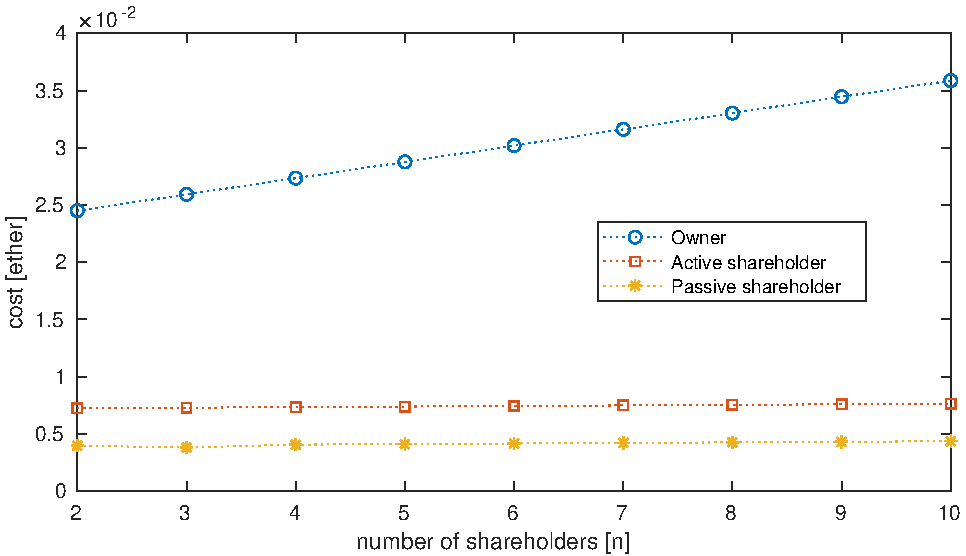
\includegraphics[height=135pt]{fig/ityt_cost_in_ether.pdf}}
	\end{comment}
	\caption{\shortname cost for each role. 1 gas = $20 \cdot 10^{-9}$ ETH; 1 ETH = 178 $\$$ }	
	\label{fig:costfigs}	
\end{figure}

\paragraph*{Test setup}
We performed two types of experiment on $\shortname$: (i) simulation of $\shortname$ smart contract instances, and (ii) execution of sMPC network protocols. 
For both cases, the size of the shares was set to 256 bits (the maximum supported by the FRESCO sMPC framework).
The tests have been executed on an dual Intel Xeon E5 server with 256 GB memory and 512 GB SSD drive running Ubuntu 18.04 LTS.

\medskip

\paragraph*{Simulation of \shortname instances}
A preliminary version of the $\shortname$ smart contract was derived by the use of FSolidM~\cite{Mavridou2017DesigningSE}, a tool which automatically generates Ethereum smart contracts code from high level Finite State Machine (FSM) representations.
To deploy, test, and debug the contract created, we relied on Brownie~\cite{brownie}, a python framework that permits to create wallets, inspect transactions and automate the execution of simulations.
To provide such functionalities, Brownie interacts with Ganache~\cite{ganache}: a local Ethereum blockchain instance used for development purposes.

The experiments mainly focused on estimating of the total cost of execution of each $\shortname$ instance. 
Figure~\ref{fig:costfigs} shows the total execution cost in gas (a proxy for the number of operations) and dollars, for each role, depending on the number of participants.
%
Due to the fact that many \shortname actions imply writing a state change to the blockchain, the first shareholder to perform the operations will incur in greater costs compared to the other ones. We name this role {\em active} shareholder.
The shareholder cost in Figure~\ref{fig:costfigs} takes into account only the calls needed to collect the reward. A shareholder that only performs these operations is named {\em passive} shareholder.
In our experiments, the active shareholder was paying approximately $0.40$ USD more (depending on the number of participants). It is easy to setup a higher reward for the {\em active} shareholder to offset the additional execution fees.
%By the previous differentiation it is possible to highlight an upper and a lower cost bound.
From the owner's perspective the total cost of execution is linear in the number of shareholders, while the contract deployment itself costs 7.39 USD.
All the costs were calculated by applying the conversion rate {$20 \cdot 10^{-9}$ ETH} and the exchange rate {1 ETH $=$ 178 USD} (as of September 12, 2019).

\medskip

\paragraph*{sMPC protocols}

The sMPC protocols were implemented using the FRESCO~\cite{FRESCO-git,damgaard2016mpc} framework.
First, we implemented a single-phase sMPC protocol compliant with the description in Section~\ref{sect:impl_mpc_brief}.
%(briefly, \owner inputs \key and gets the commitments of all shares; while each $\shareholder$ inputs a seed and receives her $\share$ and the commitment of the key).
The sMPC algorithm receives as input the key \key from the owner \owner and the seeds from all the participants. Then, it creates the polynomial and generates random shares. After that, the algorithm proceeds in computing the commitments with the MiMC function.
%In doing so, we adopted both the two existing sMPC implementation approaches: (i) the one based on binary arithmetic (i.e., to compute the Shamir polynomial), and (ii) the one based on modular arithmetic (i.e., to compute the MiMC hash commitments).
As illustrated in Figure~\ref{fig:timecomp}a, strictly adhering to this protocol leads to a quick performance degradation, as the number of shareholders increases. This is due to the fact that computing MiMC hashes among several participants is computationally expensive and highly affected by network latency (the participants have to exchange several messages to carry out even simple operations in the sMPC setting).

\begin{figure}[t]
	\centering
	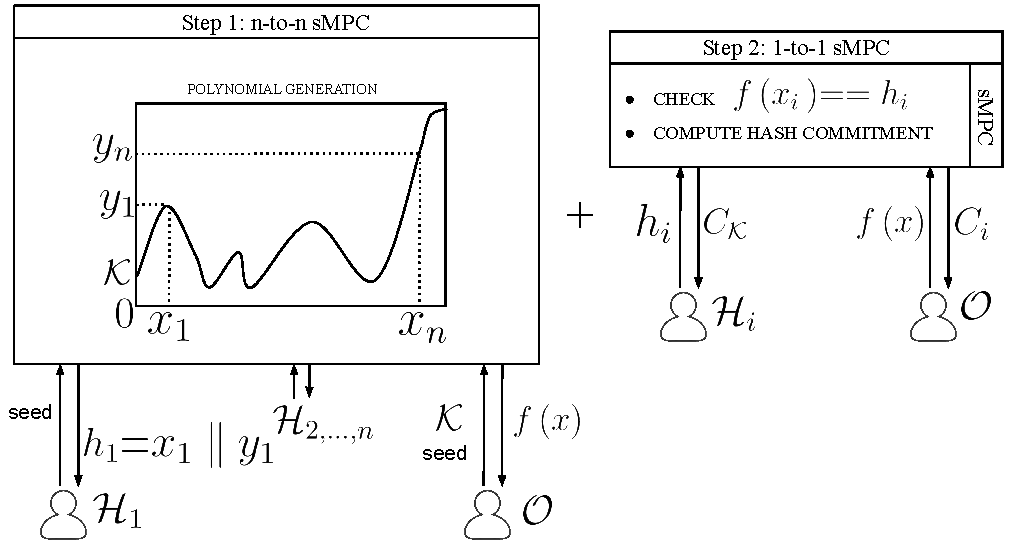
\includegraphics[width=0.9\columnwidth]{fig/mpc_rev_2}
	
	\caption{Two-phases sMPC protocol: step 1 jointly computed between all the parties, step 2 between owner and each shareholder}\vspace*{-2pt}
	\label{fig:mpc2}%
\end{figure}

To improve performance, we implemented a two-phases sMPC protocol. 
This in turn is made up of two subsequent sMPC protocols:
\begin{itemize}
	\item {\em Step 1} n-to-n sMPC jointly computed by all participants. The owner inputs \key and receives the polynomial function $f\left( x \right)$ randomly generated inside the sMPC, while each shareholder inputs a seed and receives her share (see Figure~\ref{fig:mpc2}). 
	\item {\em Step 2} 1-to-1 sMPC computed between the owner and each shareholder $i$. The owner inputs $f\left( x \right)$, and receives the commitment of the $i$-th share, $\commitment_i$, while the $i$-th shareholder inputs her share $\share_{i}$, and receives the commitment of the key (see Figure~\ref{fig:mpc2}). It is easy to verify inside the sMPC that neither the owner nor the shareholder changed the value received as a result of the first step.
\end{itemize}


\begin{figure*}[t]
	\centering
	\subfloat[Single-phase vs Two-phases]{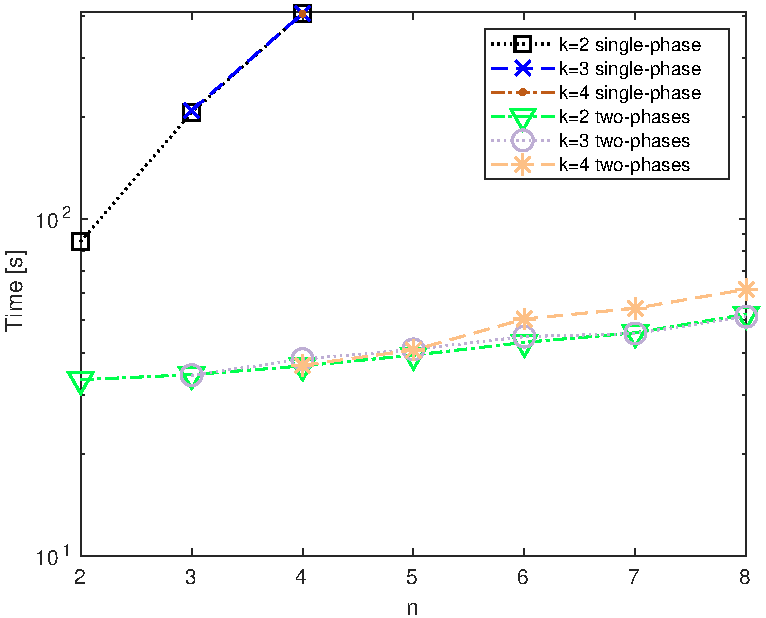
\includegraphics[height=134pt]{fig/1a.pdf}}
	\hfill
	\subfloat[Two-phases time detail]{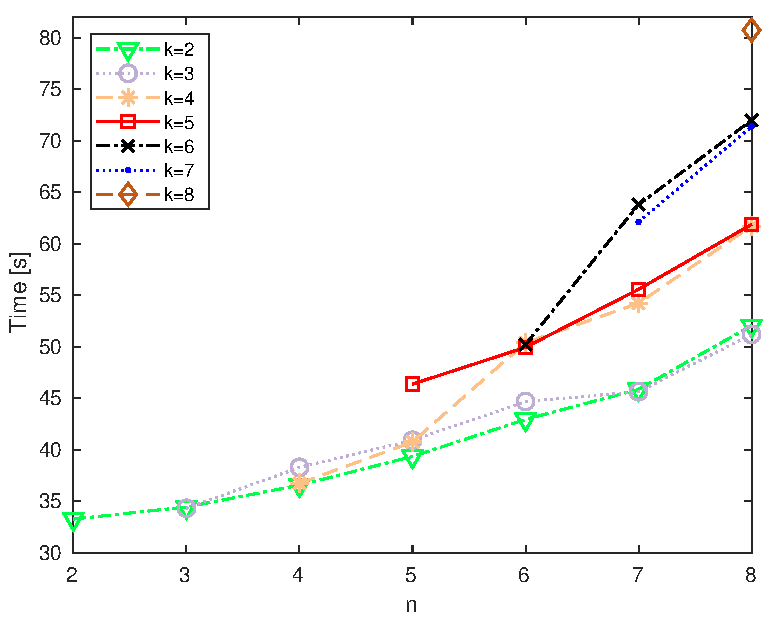
\includegraphics[height=134pt]{fig/1b.pdf}}
	\hfill
	\subfloat[Two-phases maximum memory usage]{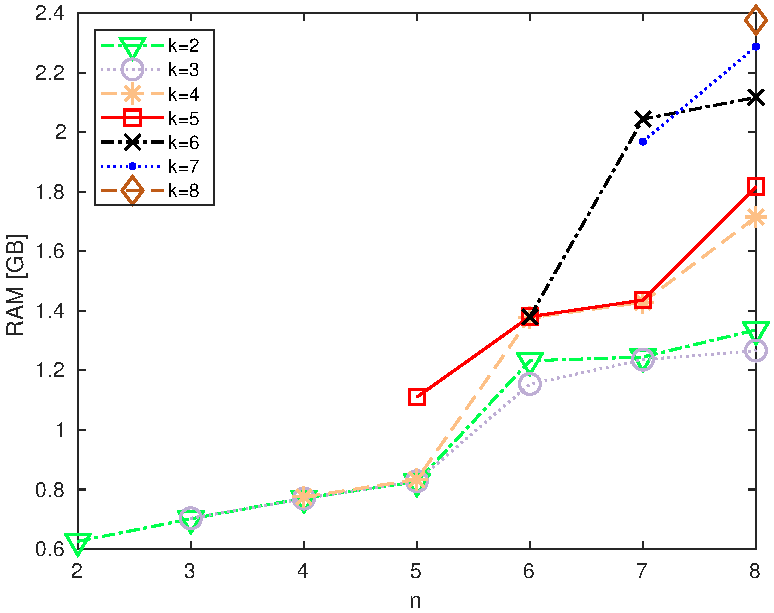
\includegraphics[height=135pt]{fig/1c.pdf}}
	\caption{sMPC execution time and maximum memory consumption for each participant, in detail: (a) comparison between single-phase and two-phases maximum execution time, (b) two-phases execution time and (c) maximum memory consumption for higher SSS polynomial degree}
	\label{fig:timecomp}
\end{figure*}


As the reader can notice, the difference between the single-phase and the two-phase sMPC lies in the calculation of the hash primitive. 
Unlike the single-phase version, the two-phases solution permits to separate the generation of the shares from the production of commitments.
The benefit that follows is that the first step is not computing intensive and can be easily computed even in a scenario with several participants, whereas the second step is always performed among two participants, thus being very practical.
The improvement of total sMPC execution time between the two variants (i.e., single-phase vs two-phases) is shown in Figure~\ref{fig:timecomp}a.
More details about the two-phases maximum execution time and maximum memory consumption in case of higher polynomial degree, for each participant, are illustrated in Figure~\ref{fig:timecomp}b and Figure~\ref{fig:timecomp}c, respectively.



\begin{figure*}[t]
	\centering
	\subfloat[]{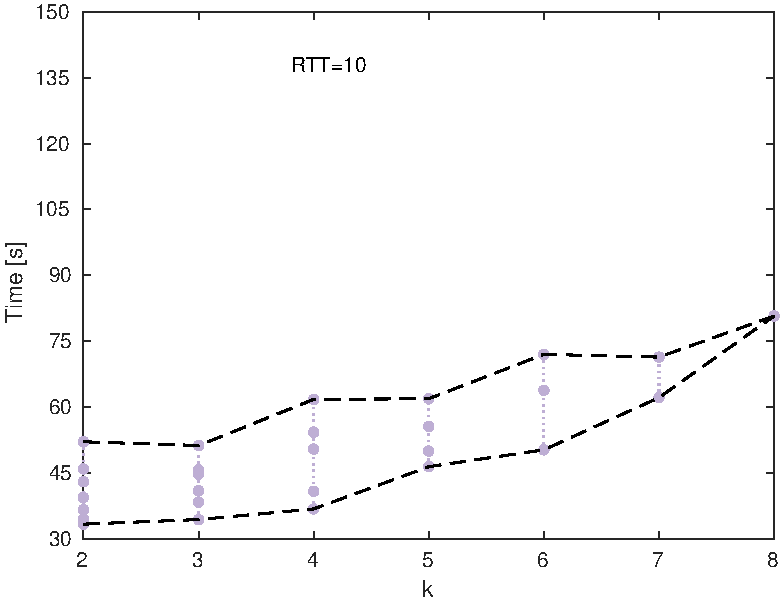
\includegraphics[height=132pt]{fig/2a.pdf}}
	\hfill
	\subfloat[]{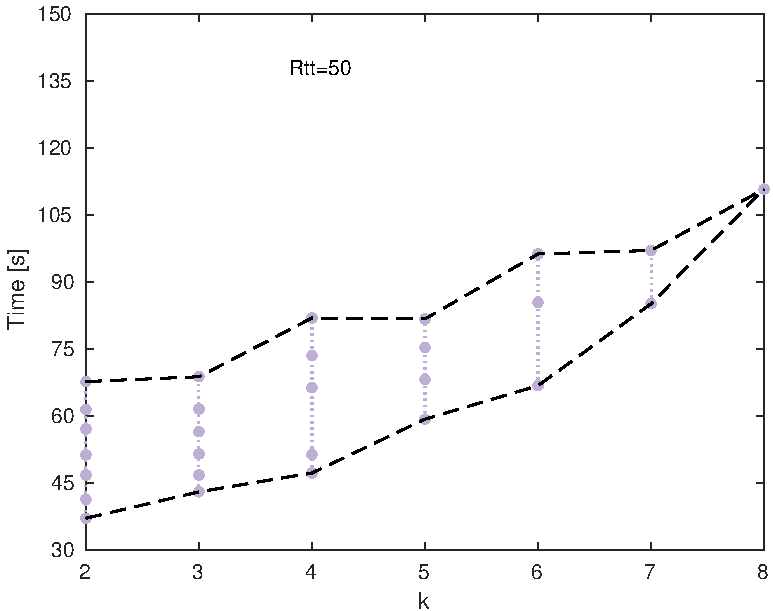
\includegraphics[height=132pt]{fig/2b.pdf}}
	\hfill
	\subfloat[]{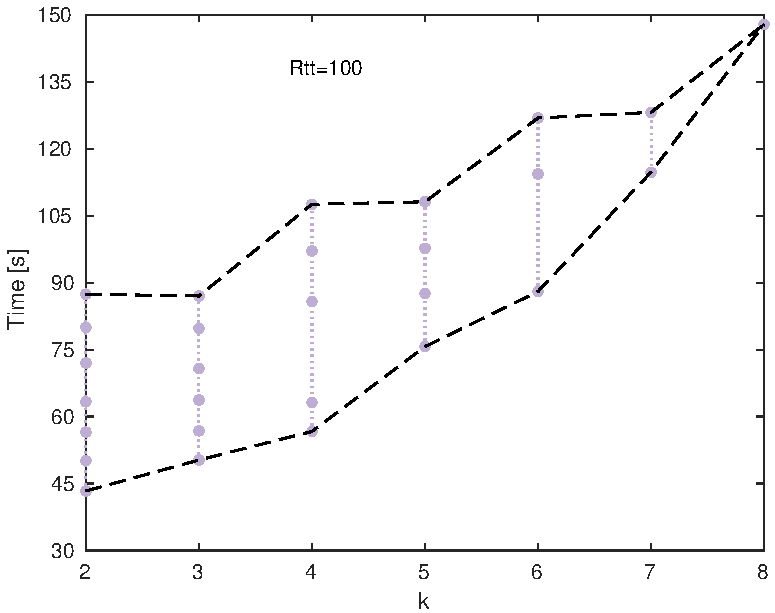
\includegraphics[height=132pt]{fig/2c.pdf}}
	\caption{sMPC total execution time for different round trip times (RTT) and polynomial degree}
	\label{fig:timertt}
\end{figure*}


For each participant, a different server was established, and the network communication round trip time (RTT) was set to 10 ms (Figure~\ref{fig:timecomp}). 
To measure the effect of RTT, we repeated the execution of all network protocols with different latency values.
Figure~\ref{fig:timertt} shows a subset of the data collected for the two-phases solution (see the repository for full detail).   
However, for an exhaustive analysis on the impact of environmental parameters over sMPC implementing secret sharing cryptography, we refer the reader to~\cite{DBLP:journals/corr/abs-1804-03548}.












